\begin{landscape}

\section{Modelo de Entidad Relación}

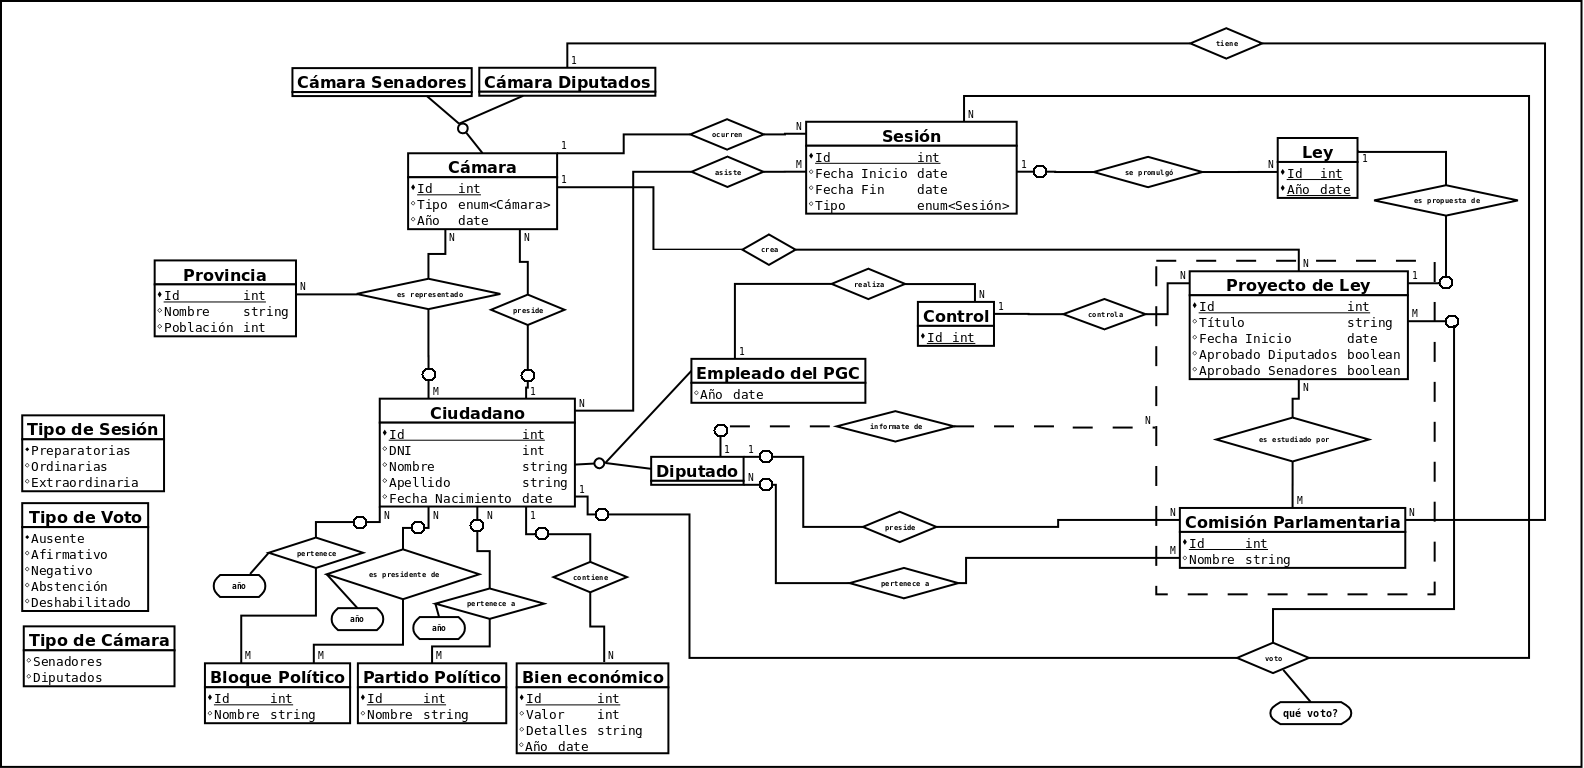
\includegraphics[width=1.6\textwidth]{CongresoDeAlgunaNacion.png}

\end{landscape}

Las restricciones que no pueden ser modeladas en el diagrama son expresadas a continuación utilizando el lenguaje natural:
\begin{itemize}
	\item Solo existe, a lo sumo, una Cámara de Diputados y otra de Senadores por año. 
	\item Por cada 33000 habitantes de una Provincia, deberá haber un Diputado que la represente en la Cámara de Diputados. 
	\item Un Legislador puede ser Diputado si tiene más de 25 años.
	\item Un Legislador puede ser Senador si tiene más de 30 años.
	\item El Vicepresidente de la Nación no es Senador.
	\item El Vicepresidente de la Nación es Presidente de la Cámara de Senadores. 
	\item El Presidente de la Cámara de Diputados debe ser Diputado de la misma, en ese año. 
	\item La Fecha de Inicio de una Sesión (menos la Extraordinaria) debe estar comprendida entre el 1 de Marzo hasta el 30 de noviembre del mismo año.	
	\item La Sesión Extraordinaria puede extender el Período Legislativo. 
	\item La Fecha de Fin de una Sesión debe estar comprendida entre el 1 de Marzo hasta el 30 de Noviembre del mismo año.
	\item La Fecha Inicio de una Sesión debe ser menor a la Fecha Fin de la misma. 
	\item Una Ley solo puede existir si su correspondiente proyecto fue aprobado por la mayoría de ambas Cámaras (de Diputados y de Senadores).
	\item Los Legisladores de una Cámara solo pueden votar en un proyecto si la misma es la de origen o ya fue aprobada por esta.
	\item En la Cámara de Diputados debe haber a lo sumo 45 Comisiones Parlamentarias.
	\item Un Diputado no puede ser presidente de dos Comisiones Parlamentarias en un mismo año.
	\item Un Diputado que sea presidente de una Comisión Parlamentaria debe pertenecer a la misma. 
	\item Un Legislador solo puede votar si tiene menos de 15 ausencias anuales, caso contrario estará deshabilitado durante ese período legislativo.
	\item Los Bienes Económicos deben ser declarados en su totalidad en cada cambio de año.
	\item Un Ciudadano que asiste a una Sesión, debe ser Legislador de la Cámara en donde ocurre la misma.
	\item No puede haber dos Legisladores del mismo Partido Político en distintos Bloques Políticos. 
	\item Existe un voto de un Legislador que no es ''ausente'' si y sólo si asistió la Sesión correspondiente.
	\item Los Legisladores que pertenecen a alguna de las Cámaras, debieron realizar una única Declaración Jurada de ese año.
	\item Un Legislador no puede pertenecer a las dos Cámaras al mismo tiempo. 
	\item Un Legislador no puede representar a más de una provincia en la misma Cámara. 
	\item Un Ciudadano sólo puede pertenecer a la Cámara de Diputados si es un Diputado.
	\item Un Ciudadano que es Empleado no puede pertenecer a ninguna de las Cámaras de ese año.	
	\item Si un Legislador asiste a una Sesión, entonces debe ser representante de la cámara en donde ocurre la misma.

\end{itemize}

\newpage

\section{Modelo Relacional}

\begin{itemize}
	\item \textbf{Cámara} \\
	id (PK) \\
	Tipo \\
	Año \\
	Presidente\_id (FK - Ciudadano)
	
	\item \textbf{Cámara Senadores} \\
	id (PK) (FK - Cámara) 
	
	\item \textbf{Cámara Diputados} \\
	id (PK) (FK - Cámara)
	
	\item \textbf{Ciudadano} \\
	id (PK) \\
	DNI \\
	Fecha Nacimiento \\
	Nombre \\
	Apellido
	
	\item \textbf{Diputado} \\
	id (PK) (FK - Ciudadano)
	
	\item \textbf{Empleado del PGC} \\
	id (PK) (FK - Ciudadano) \\
	Año
	
	\item \textbf{Provincia} \\
	id (PK) \\
	Nombre \\
	Población
	
	\item \textbf{Representaciones} \\
	Ciudadano\_id (PK) (FK - Ciudadano) \\
	Cámara\_id (PK) (FK - Cámara) \\
	Provincia\_id (PK) (FK - Provincia) 
		
	\item \textbf{Bloque Político} \\
	id (PK) \\
	Nombre
	
	\item \textbf{Bloques Políticos\_Ciudadanos\_Presidentes} \\
	Ciudadano\_id (PK) (FK - Ciudadano) \\
	Bloque Político\_id (PK) (FK - Bloque Político)\\
	Año (PK)
	
	\item \textbf{Bloques Políticos\_Ciudadanos\_Integrantes} \\
	Ciudadano\_id (PK) (FK - Ciudadano) \\
	Bloque Político\_id (PK) (FK - Bloque Político)\\
	Año (PK)
	
	\item \textbf{Partido Político} \\
	id (PK) \\
	Nombre 
	
	\item \textbf{Partidos Políticos\_Ciudadanos} \\
	Ciudadano\_id (PK) (FK - Ciudadano) \\
	Partido Político\_id (PK) (FK - Partido Político)\\
	Año (PK)
	
	\item \textbf{Sesión} \\
	id (PK) \\
	Fecha\_inicio \\
	Fecha\_fin \\
	Cámara\_id (FK - Cámara) \\
	Tipo
	
	\item \textbf{Control} \\
	id (PK) \\
	Empleado\_id (FK - Empleado del PGC)
	
	\item \textbf{Proyecto de Ley} \\
	id (PK) \\
	Fecha inicio \\
	Cámara\_id (FK - Cámara) \\ 
	Título \\
	Control\_id (FK - Control) \\
	Aprobado Diputados \\
	Aprobado Senadores
	
	\item \textbf{Ley} \\
	id (PK) \\
	Año \\
	Sesión\_id (FK - Sesión) \\
	Proyecto de Ley\_id (FK - Proyecto de Ley)
	
	\item \textbf{Votos} \\
	Ciudadano\_id (PK) (FK - Ciudadano) \\
	Sesión\_id  (FK - Sesión) \\
	Proyecto de Ley\_id (PK) (FK - Proyecto de Ley) \\
	Tipo de Voto
	
 	\item \textbf{Comisión} \\
 	id (PK) \\
 	Nombre \\
 	Cámara Diputados\_id (FK - Cámara Diputados) \\
 	Presidente\_id (FK - Diputado)
 	
	\item \textbf{Integrantes\_Comisiones} \\
	Diputado\_id (PK) (FK - Diputado) \\
	Comisión\_id (PK) (FK - Comisión) 
	
	\item \textbf{Proyectos de Ley\_Comisiones} \\
	Proyecto de Ley\_id (PK) (PK - Proyecto de Ley) \\
	Comisión\_id (PK) (PK - Comisión) \\
	Informante\_id (PK - Diputado)
	
	\item \textbf{Asistencias} \\
	Ciudadano\_id (PK) (FK - Ciudadano) \\
	Sesión\_id (PK) (FK - Sesión)
		
	\item \textbf{Bien Económico} \\
	id (PK) \\
	Valor \\
	Detalles \\ 
	Año \\
	Ciudadano\_id (FK - Ciudadano)
	
\end{itemize}

\newpage

\section{Supuestos asumidos}
La abstracción de la realidad reduce a los cuidadanos para que sean únicamente aquellos que trabajan en la legislatura de la Nación.


Por otro lado, se asume que un Proyecto de Ley solo puede ser controlado por un Control. 


En ciertas relaciones, se decidió guardar la historia entre las entidades que participan de las mismas, a pesar de que no esté especificado claramente en el enunciado.


Un Legislador es un Ciudadano que puede ser tanto un Diputado como un Senador.


Se consideró como tipo de voto, además de ''positivo'' , ''negativo'' y ''abstención'', los de ''ausente'' y ''deshabilitado'' por motivos de diseño.